% style notes
% - \,percent not \%

\documentclass[12pt, preprint]{aastex}
\usepackage{bm, graphicx, subfigure, amsmath, morefloats}

% words
\newcommand{\project}[1]{\textsl{#1}}
\newcommand{\thecannon}{\project{The~Cannon}} 
\newcommand{\tc}{\project{The~Cannon}} 
\newcommand{\apogee}{\project{APOGEE}}
\newcommand{\apokasc}{\project{APOKASC}}
\newcommand{\aspcap}{\project{ASPCAP}}
\newcommand{\corot}{\project{Corot}}
\newcommand{\kepler}{\project{Kepler}}
\newcommand{\gaia}{\project{Gaia}}
\newcommand{\gaiaeso}{\project{Gaia--ESO}}
\newcommand{\galah}{\project{GALAH}}
\newcommand{\most}{\project{MOST}}
\newcommand{\code}[1]{\texttt{#1}}
\newcommand{\documentname}{\textsl{Article}}

\newcommand{\teff}{\mbox{$\rm T_{eff}$}}
\newcommand{\kms}{\mbox{$\rm kms^{-1}$}}
\newcommand{\feh}{\mbox{$\rm [Fe/H]$}}
\newcommand{\xfe}{\mbox{$\rm [X/Fe]$}}
\newcommand{\alphafe}{\mbox{$\rm [\alpha/Fe]$}}
\newcommand{\mh}{\mbox{$\rm [M/H]$}}
\newcommand{\logg}{\mbox{$\rm \log g$}}
\newcommand{\noise}{\sigma_{n\lambda}}
\newcommand{\scatter}{s_{\lambda}}
\newcommand{\pix}{\mathrm{pix}}
\newcommand{\rfn}{\mathrm{ref}}
\newcommand{\rgc}{\mbox{$\rm R_{GC}$}}
\newcommand{\rgal}{\mbox{$\rm R_{GAL}$}}
\newcommand{\vgal}{\mbox{$\rm V_{GAL}$}}

% math and symbol macros
\newcommand{\set}[1]{\bm{#1}}
\newcommand{\starlabel}{\ell}
\newcommand{\starlabelvec}{\set{\starlabel}}
\newcommand{\mean}[1]{\overline{#1}}
\newcommand{\given}{\,|\,}
%\newcommand{\teff}{\mbox{$\rm T_{eff}$}}
%\newcommand{\kms}{\mbox{$\rm kms^{-1}$}}
%\newcommand{\feh}{\mbox{$\rm [Fe/H]$}}
%\newcommand{\xfe}{\mbox{$\rm [X/Fe]$}}
%\newcommand{\alphafe}{\mbox{$\rm [\alpha/Fe]$}}
%\newcommand{\mh}{\mbox{$\rm [M/H]$}}
%\newcommand{\logg}{\mbox{$\rm \log g$}}
%\newcommand{\noise}{\sigma_{n\lambda}}
%\newcommand{\scatter}{s_{\lambda}}

% math
\newcommand{\numax}{$\nu_{\max}$}
\newcommand{\deltanu}{$\Delta\nu$}
\bibliographystyle{apj}

\begin{document}

\title{The Metallicity Distribution of Bulge Stars}
\author{M.~Ness\altaffilmark{1},
K. Freeman\altaffilmark{1},
\textbf{others?}}
\altaffiltext{1}{Max-Planck-Institut f\"ur Astronomie, K\"onigstuhl 17, D-69117 Heidelberg, Germany}
\altaffiltext{2}{Mt Stromlo}
\email{ness@mpia.de}


\begin{abstract}%

\end{abstract}


\section{The global MDF of the bulge of the Milky Way} 
1. Global MDF: - Discussion on the overall metallicity, gradients \\

\section{Multiple Stellar Populations in the Galactic Bulge} 


2. Formation models and the MDF: - Discussion of how models relate to observable
trends in the MDF
3. Multiple bulge populations: - Discussion on multiple populations with different
groups associating them to different origins

\section{The Bulge in the plane mapped by APOGEE}


%run -i makemeans_vel_smaller3.py
%makefig(feh3,-0.65,0.2,1,2, "$|$[Fe/H]$|$ (dex)", 'test')
\begin{figure}[h!]
    \begin{subfigure}[b]{1.1\textwidth}
    \centering
    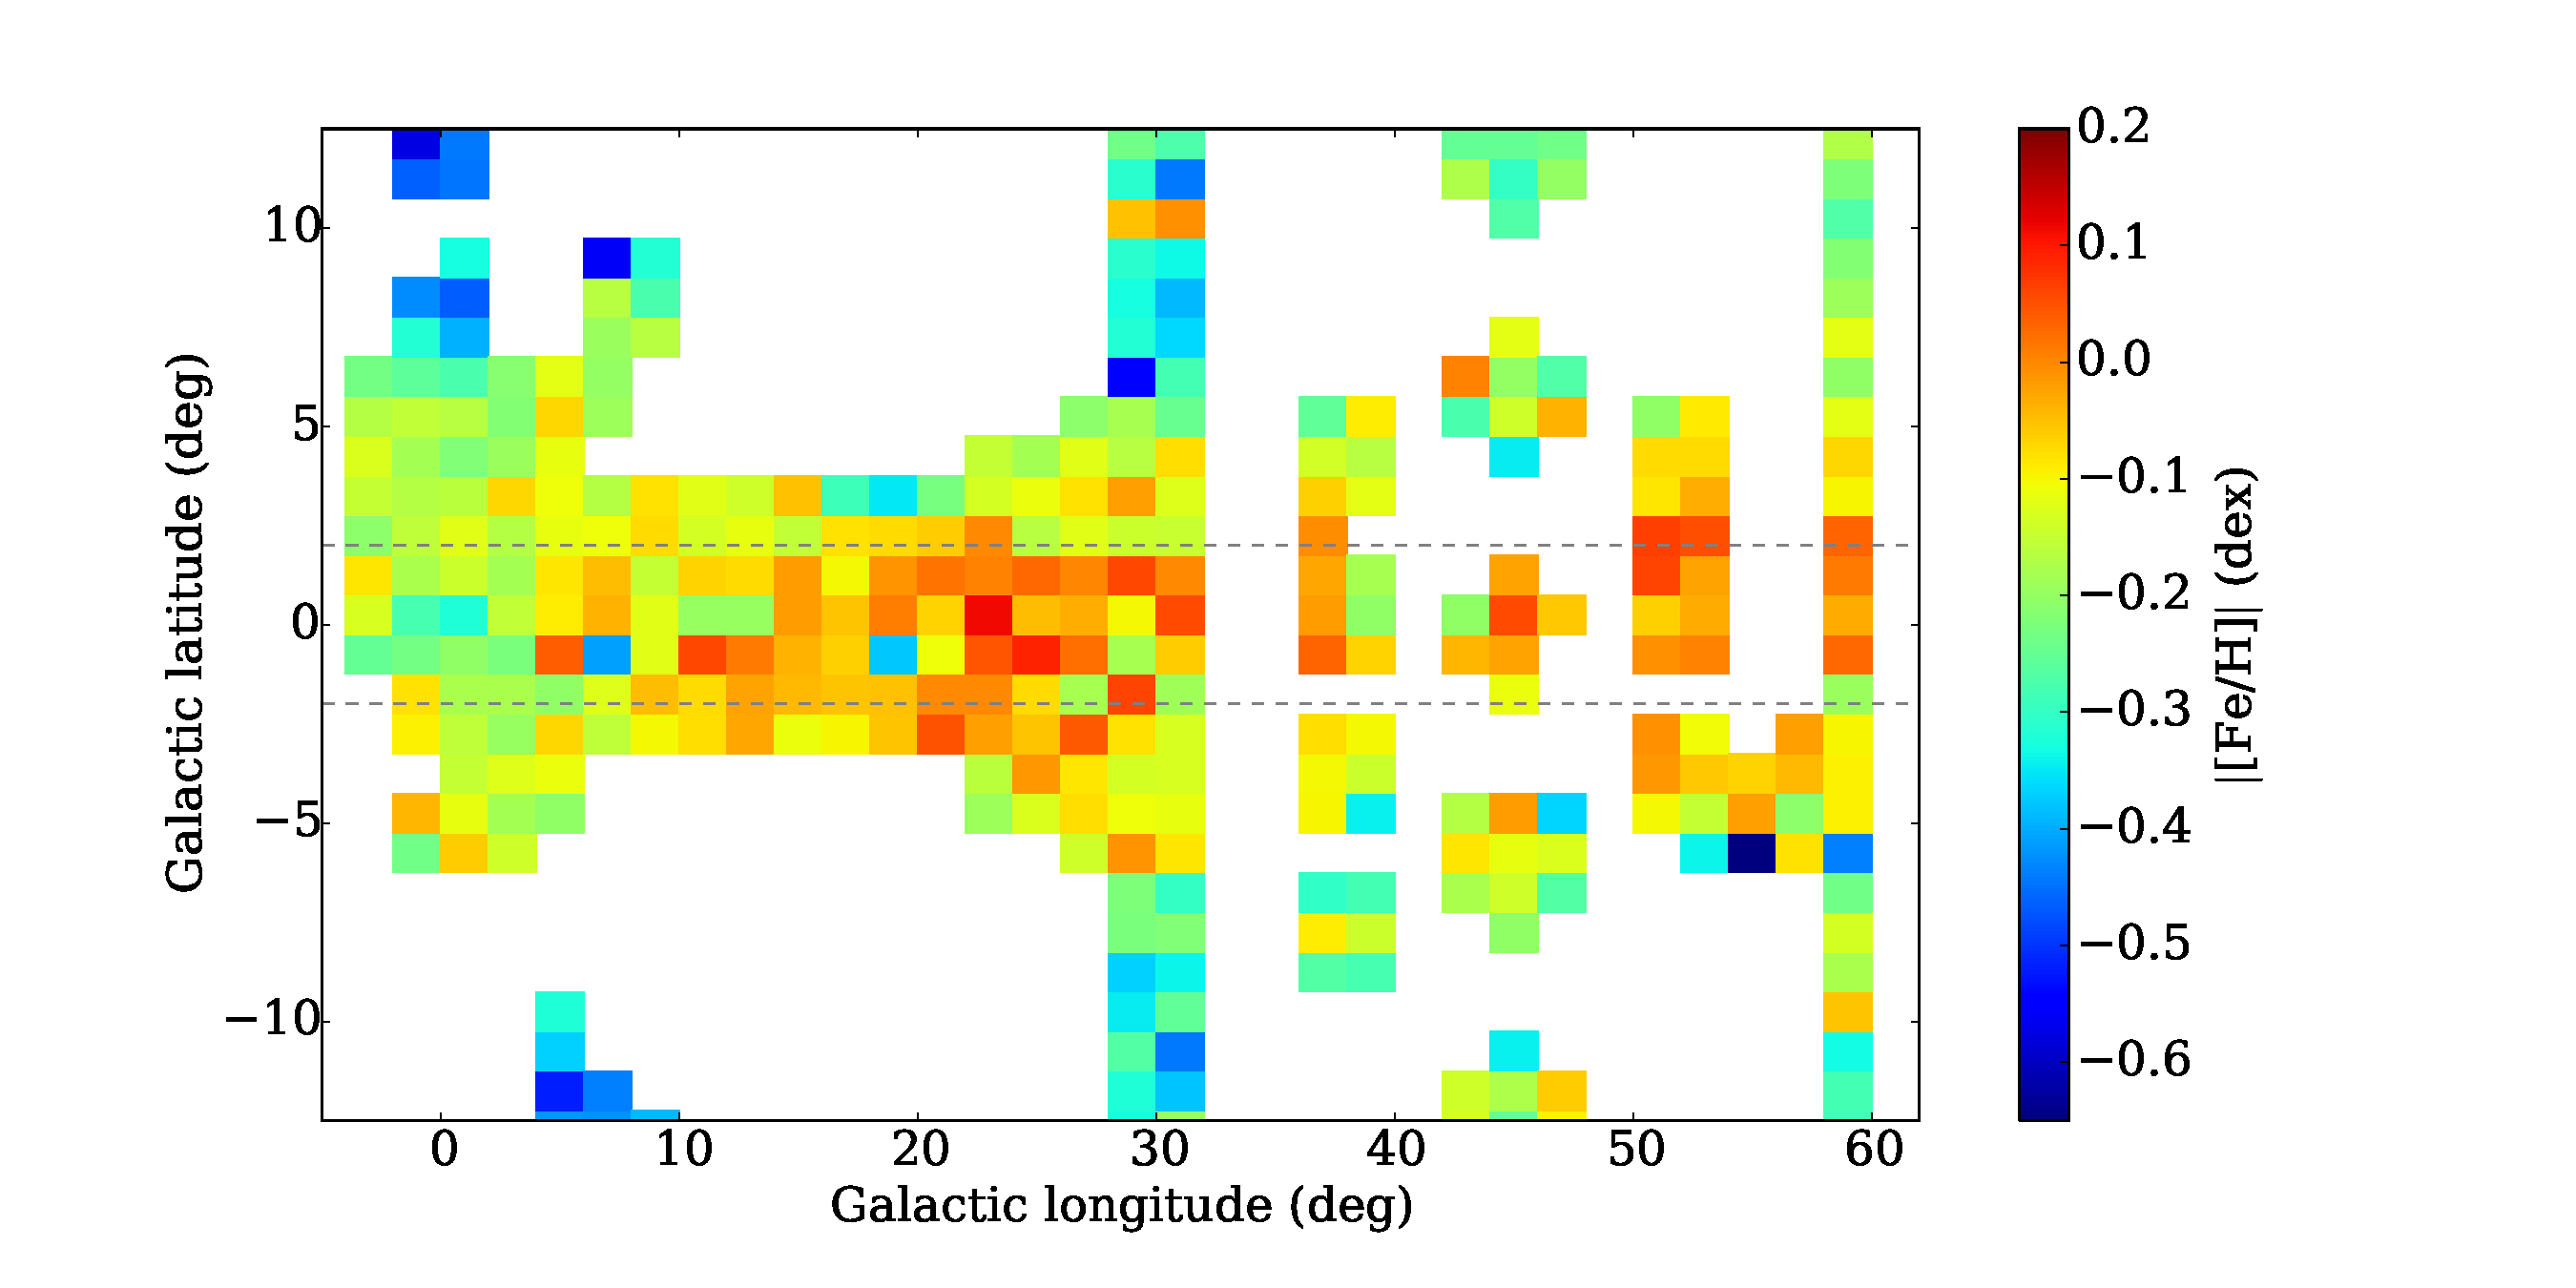
\includegraphics[width=0.8\linewidth]{fehmap.pdf}%{fehtest2_1_1.png}
    %{feh_2_1.png}
\caption{}
  \end{subfigure}%
 % \quad'
 
  \begin{subfigure}[b]{1.1\textwidth}
    \centering
    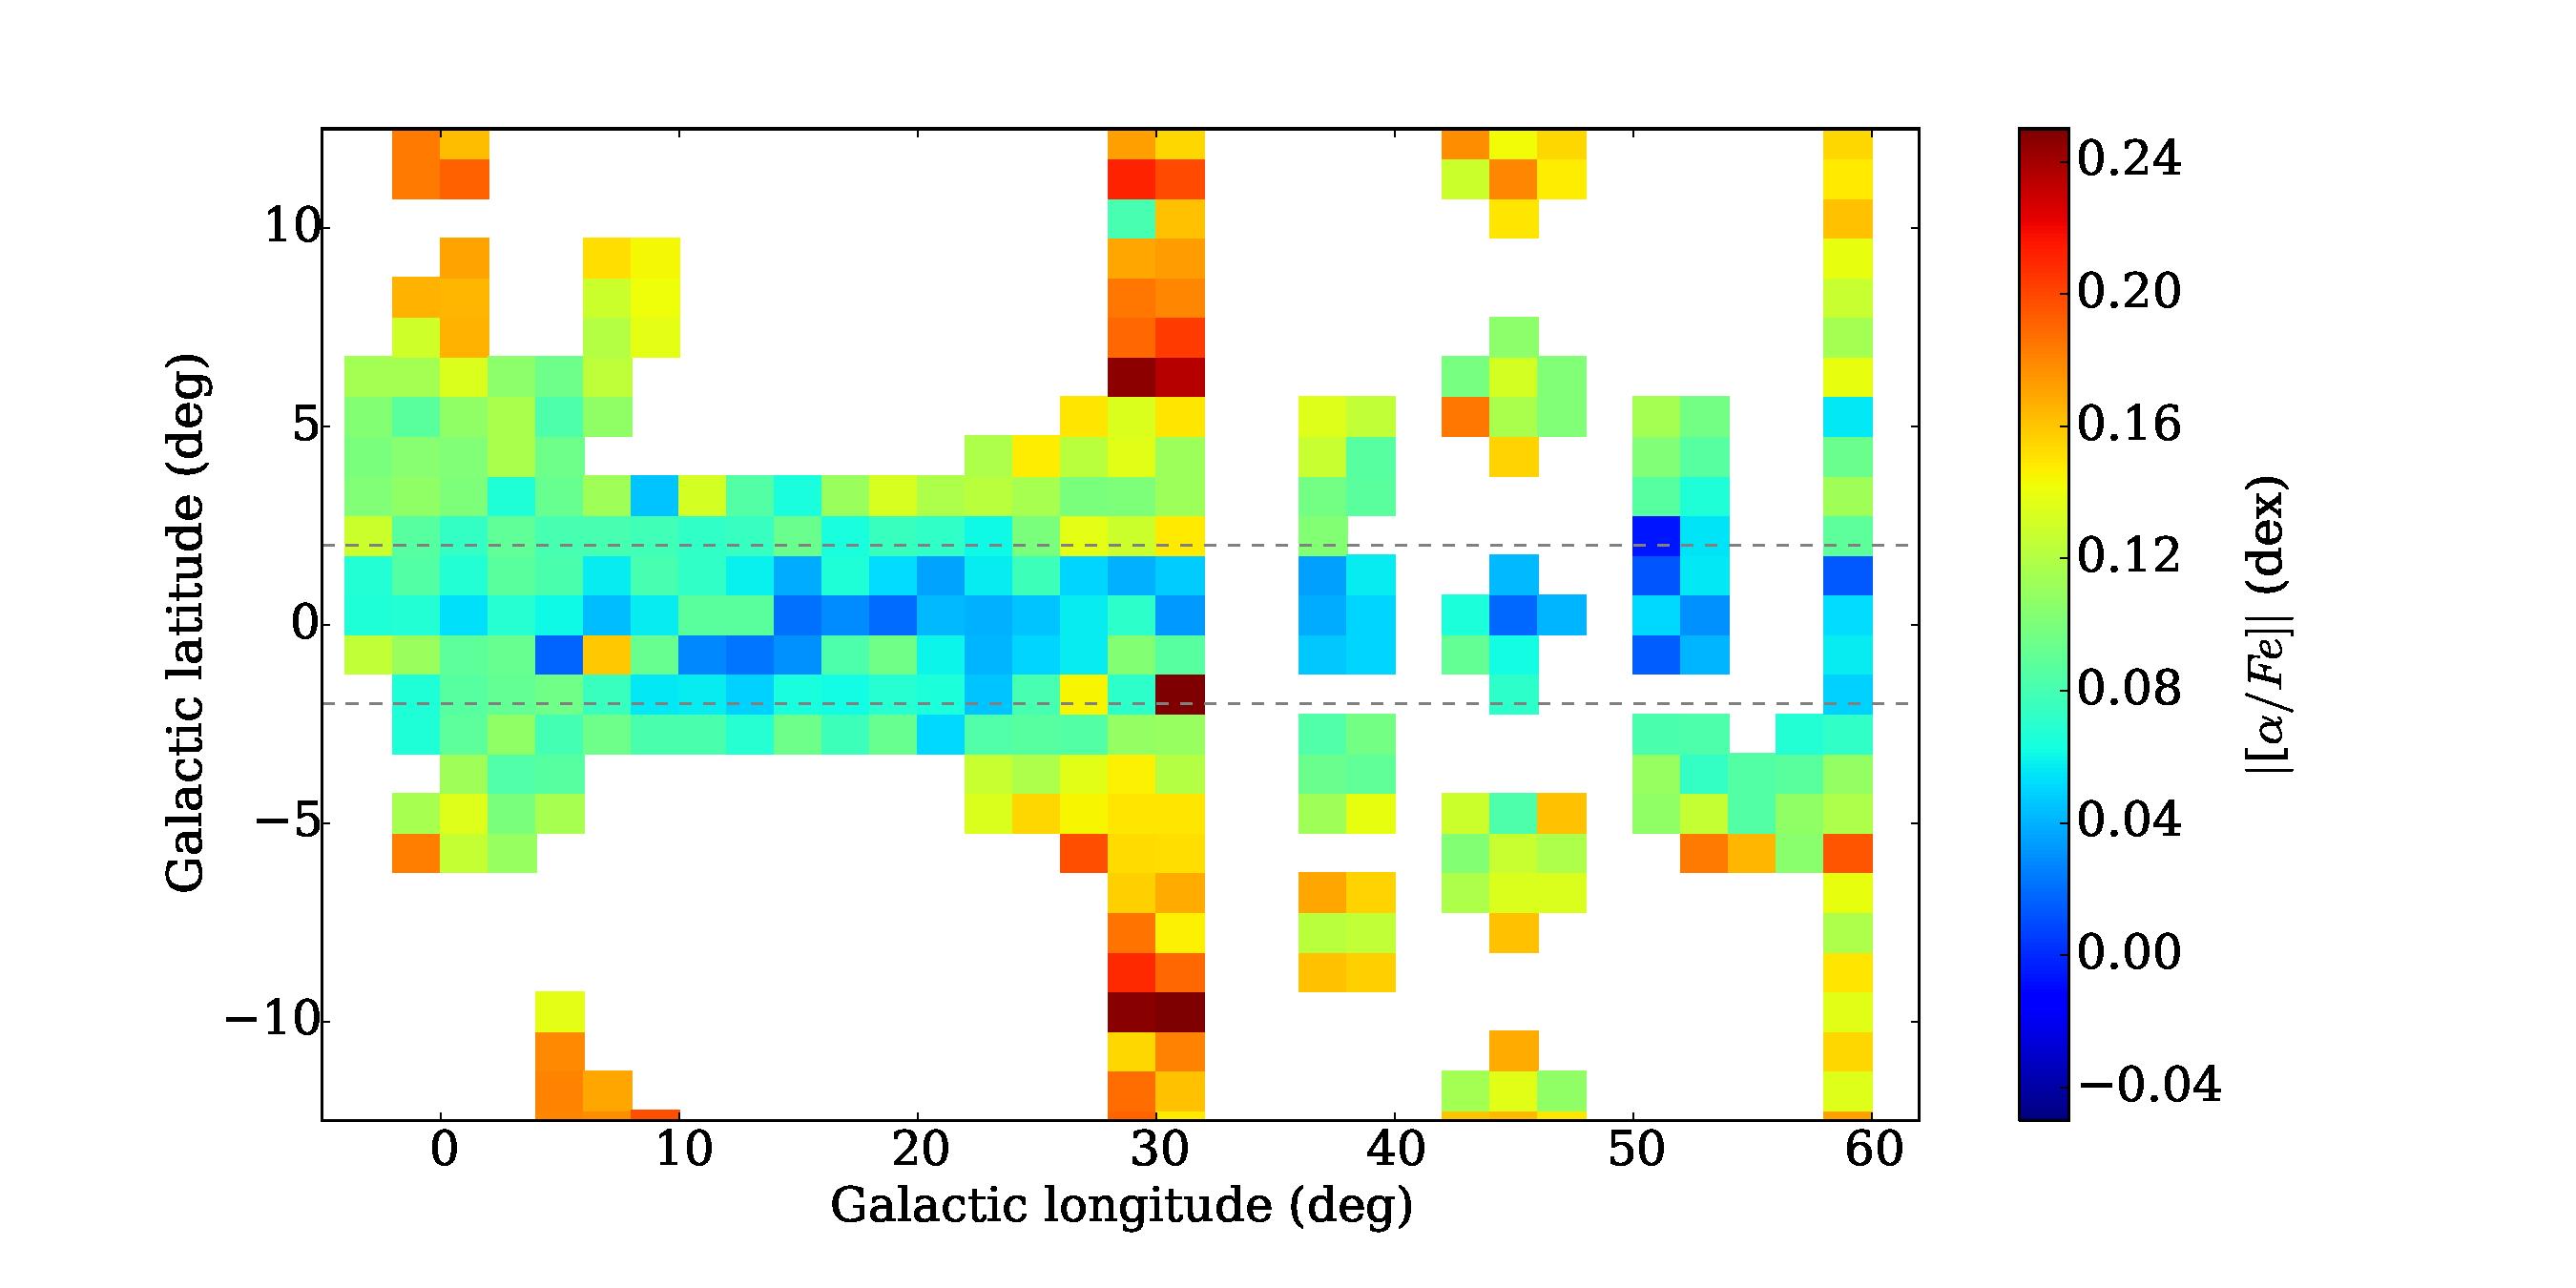
\includegraphics[width=0.8\linewidth]{alphamap.pdf}%{alphatest_1_1.png}
    %{feh_2_1.png}{alpha_2_1.png}  \\
\caption{} 
\end{subfigure}
  \caption{(a) \feh and (b) \alphafe maps for the 13,000 bulge and disk stars spanning heliocentric distances of 4--12  kpc. The dashed line indicates the scale height of the 180~pc thin bar identified by \citet{Wegg2015}.}
  \label{fig:metals}
\end{figure}



4. The MFD in the plane: - i.e. new results from APOGEE that are in hand from
analysis of public data.
\section{Kinematics of the bulge as a function of \feh}

5. Disentangling populations with kinematics, individual abundances and proper
motions: - how the additional phase-space parameters can be used to differentiate
formation histories

\section{The metal poor \feh\ $<$ --1.0 population in the bulge} 

6. The metal poor \feh $<$ -1.0 population in the bulge: - Discussion about the
RR Lyrae distribution and also what the metal poor stars in the inner region may be: distinct bulge population versus halo population.

\section*{Acknowledgments}
It is a pleasure to thank ABandC.


\bibliography{tc.bib}

\end{document}
